\documentclass[]{article}
\usepackage{enumitem}
\usepackage{siunitx}
\usepackage{graphicx}

%opening
\title{Assignment 1:  Error Analysis}
\author{K. Hendrick}
\date{}

\begin{document}

\maketitle


\begin{enumerate}
\item
\begin{enumerate}[label=(\alph*)]
\item Measured height $ h = 5.03 \pm 0.04$ m
\item Measured time $ t = 1.5 \pm 1 $ s
\item Measured charge $ q = -3.21x10^{-19} \pm 0.27x10^{-19}$ C
\item Measured distance $ d = 5.6x10^{-7} \pm 0.7x10^{-7} $ m
\item Measured momentum $ p = 3,267 \pm 42 $ gcm/s

\end{enumerate}
\item
\begin{enumerate}[label=(\alph*)]
\item Given a set of 5 measurements of a liquid's density 1.8, 2.0, 2.0, 1.9, and 1.8, the average density is

 \begin{center}$d_{ave} = \frac{1.8+2.0+2.0+1.9+1.8}{5}$. 
 \end{center}
 
To find the uncertainty from such a small data set, I found the standard deviation

\begin{center}
$\Delta d = \frac{\sqrt{\sum_{i=1}^{N}|d_i^2 - d_{ave}^2|}}{N-1} $
\end{center}
Substituting in the values from our given data set, this yields

\begin{center}
$\Delta d = \frac{\sqrt{|(3.24-3.61)| + |(4.0-3.61)| + |(4.0-3.61)| + |(3.61-3.61)| + |(3.24-3.61)|}}{4} $

$\Delta d = \frac{\sqrt{1.52}}{4} = 0.31$

This gives our result for the liquid's density and uncertainty $ d = 1.9 \pm 0.31 \frac{g}{cm^3}$
\end{center}
\item The student's estimate was within one standard deviation of the accepted value. The percent error in their calculation was 

\begin{center}
\% error $= \frac{accepted - measured}{accepted}*100 = \frac{1.85-1.9}{1.85}*100 =2.7\%$ 
\end{center}
\end{enumerate}
\item
The equation for the volume of a sphere of radius r is 
\begin{center}
$v = \frac{4}{3}\pi r^3$
\end{center}
To find the uncertainty for a sphere of radius $r = 2.0 \pm 0.1 m$, we find 
\begin{center}
$\Delta v = \sqrt{(\frac{\partial v}{\partial r} \Delta r)^2}$ 
\end{center}

We take the appropriate partial derivative of the volume function to get 

\begin{center}
$ \Delta v= \sqrt{(4 \pi r^2 \Delta r)^2}$
\end{center}
Which for our given r, $\Delta v = 5.0 m^3$. Thus, our sphere has volume 
\begin{center}
$ V_{sphere} = \frac{4}{3} \pi r^3 \pm \Delta v$ $ m^3 = 33.5 \pm 5.0 m^3$
\end{center}
\item
Given the equation $q = xy + \frac{x^2}{y}$ with $x = 6.0 \pm 0.2$ and $y = 3.0 \pm 0.1$, we can find our uncertainty 
\begin{center}
$\Delta q = \sqrt{(\frac {\partial q}{\partial x} \Delta x)^2 + (\frac{\partial q}{\partial y} \Delta y)^2}$

$\frac{\partial q}{\partial x} = y + 2xy^{-1}$ and $\frac{\partial q}{\partial y} = x-xy^{-2}$

$\Delta q = \sqrt{(y + 2xy^{-1} \Delta x)^2 + (x-xy^{-2} \Delta y)^2}$

$\Delta q = \sqrt{2.21} = 1.49$
\end{center}

We can now solve for q with our uncertainty
\begin{center}
$q = 30.0 \pm 1.5$
\end{center}

\item
\begin{enumerate}[label=(\alph*)]
\item \begin{figure}
  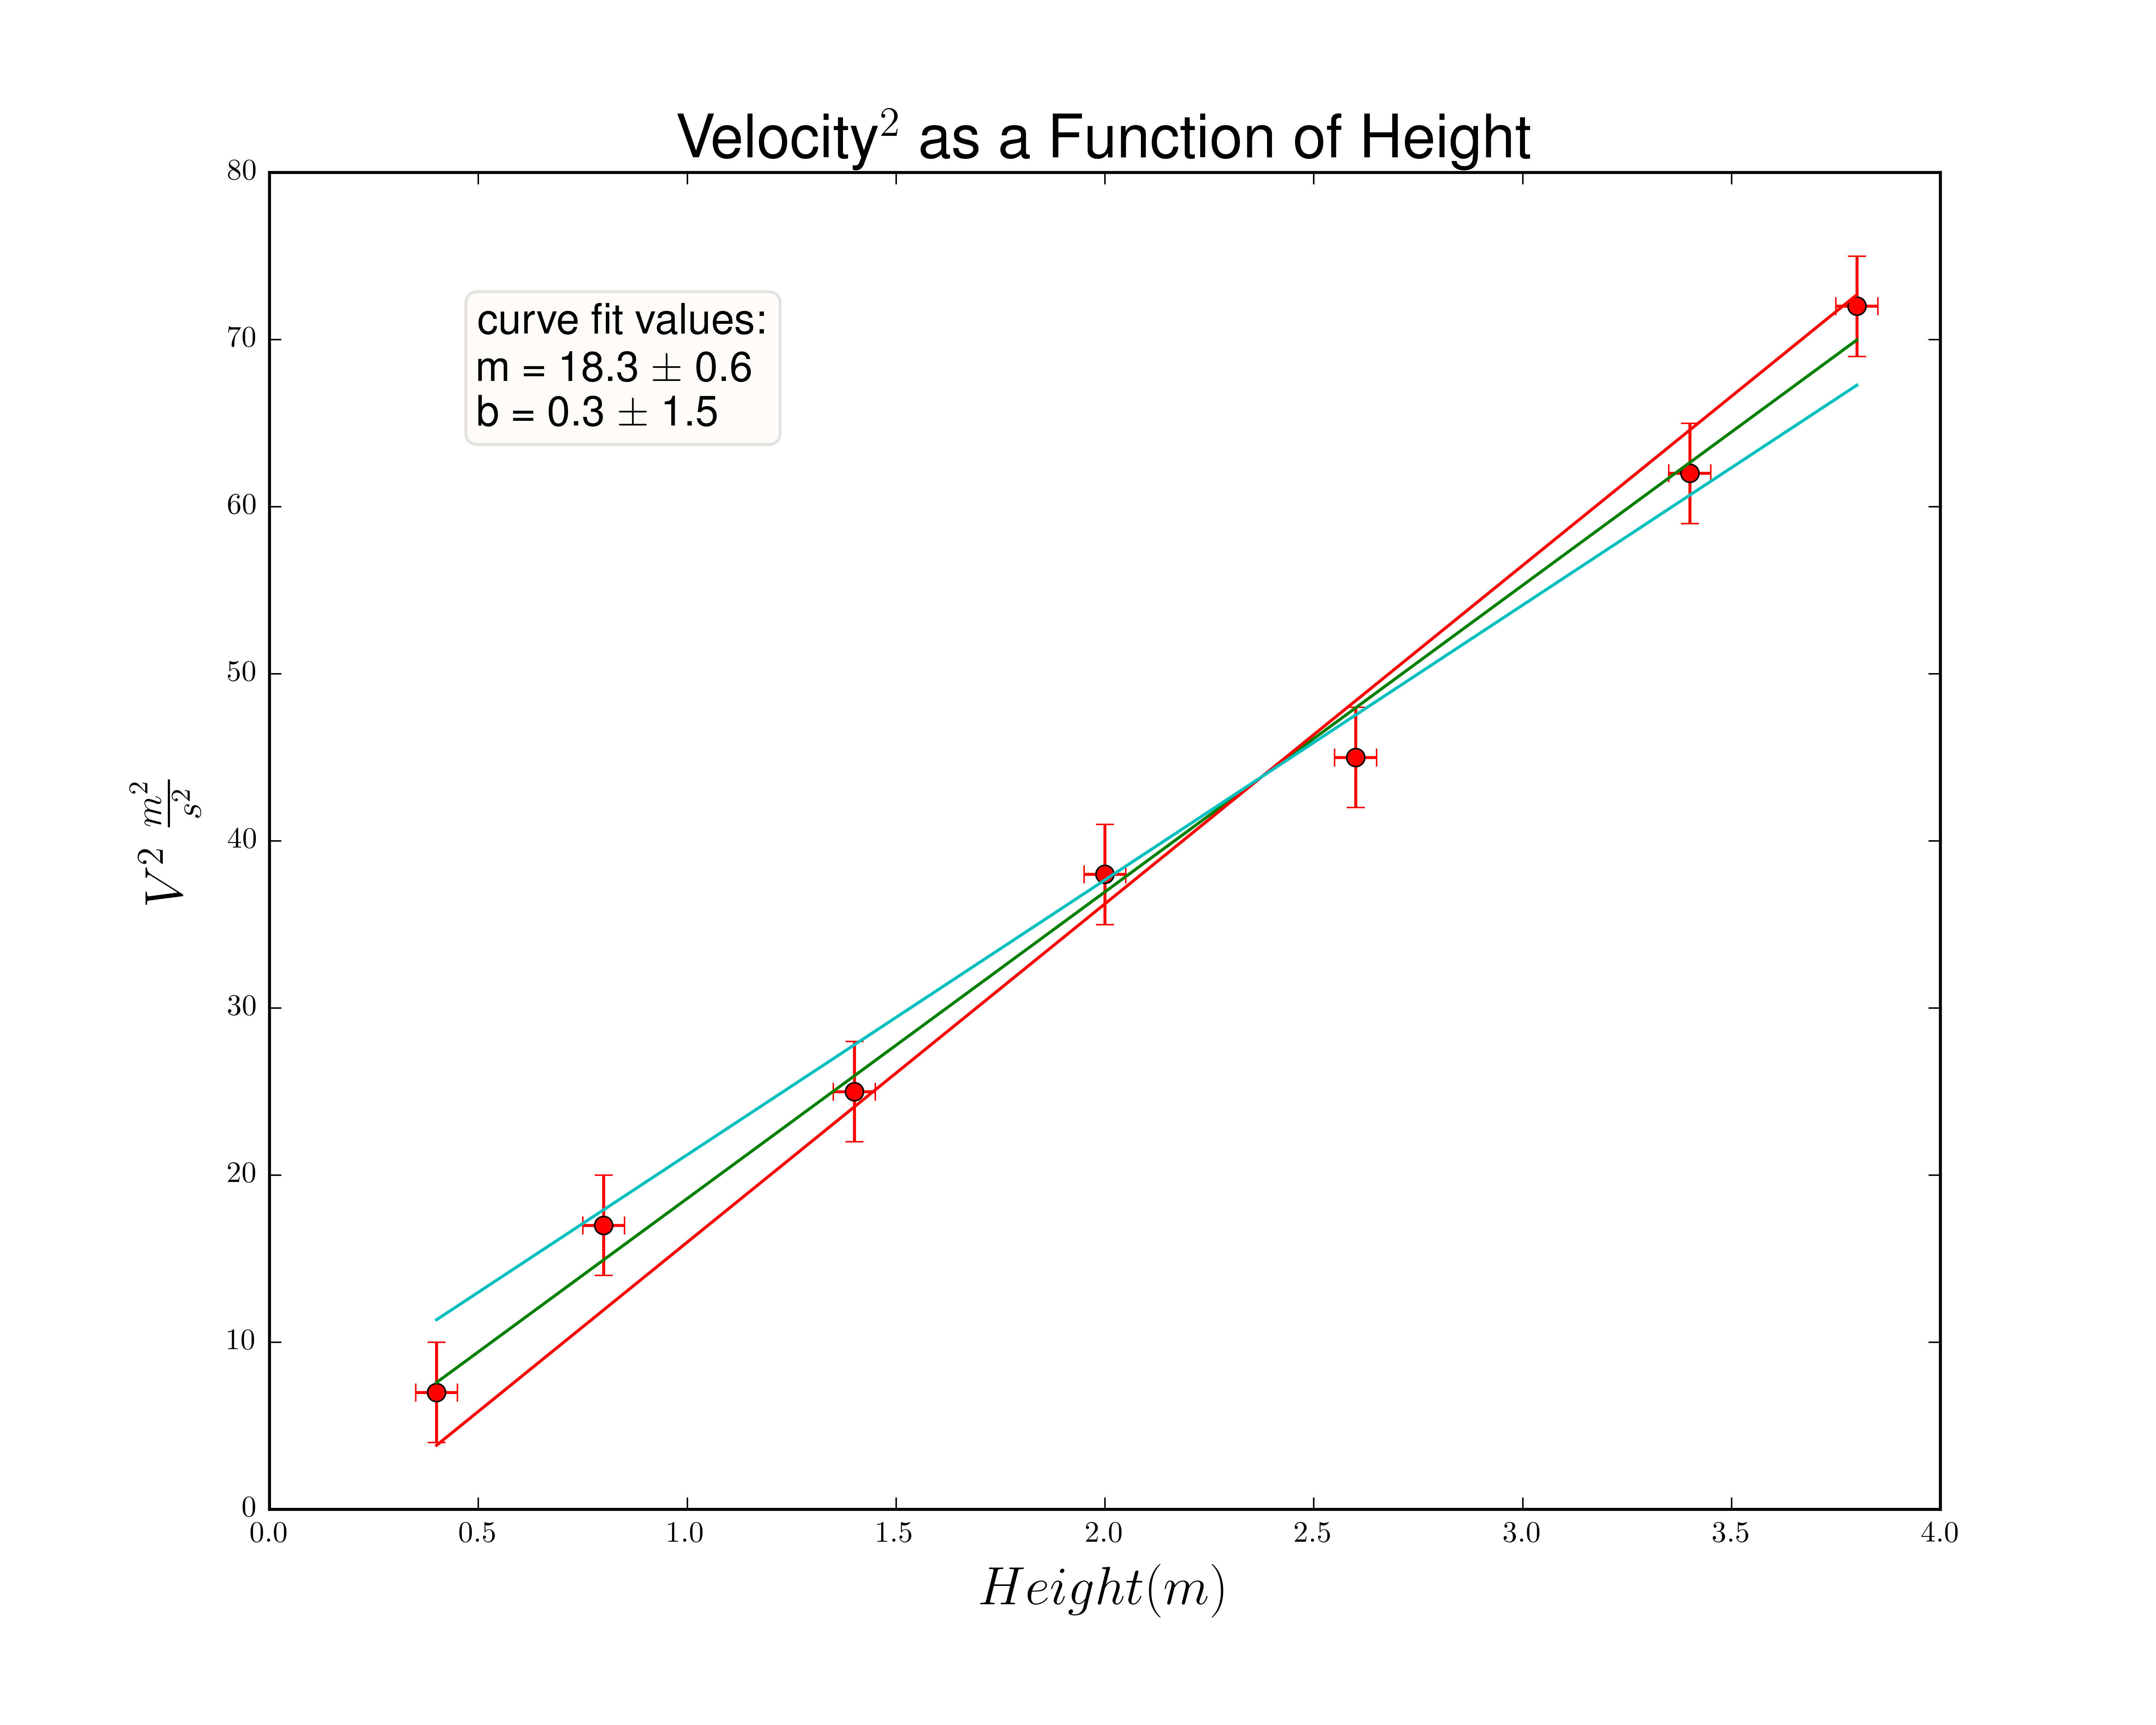
\includegraphics[width=\linewidth]{a1plot.png}
  \caption{Plot of $velocity^2$ vs $height$}
  \label{fig:Plot}
\end{figure}

Figure \ref{fig:Plot} shows the python generated plot of the square of the velocity of a vertically thrown stone as a function of its height.

The plot shows a linear relationship between the height and square of the velocity, which is consistent with $v^2 \propto h$.
\item The above plot created through python has a slope of $m = 18.3 \pm 0.6$. As $2g=19.6$, this is fairly close, but doesn't fall within the uncertainty given by the code. It might be that for such a small sample set, a different method of calculating the uncertainty might have been more appropriate.
\end{enumerate}
\end{enumerate}
\end{document}
